\chapter{Disskusion}
Dieser Versuch bestand aus 4 Aufgaben. Wir wollen alle nacheinander Zusammenfassen und anschließend Disskutieren. Zum Schluss werden noch Kritiken geäußert.
\section{Zusammenfassung}
Erstmal die Zusammenfassung der Aufgaben.
\subsection*{Aufgabe 1}
In dieser Aufgabe sollte das Osziloskop kennengelernt werden. Es wurde ein Funktionengenerator an den ersten Kanal des Oszilloskopes geschlossen, das Signal war eine Sinuskurve. Wir haben die meisten Funktionen ausprobiert und das Osziloskop gut kennengelernt. (Es wird hierzu keine Disskusion geben).

\subsection*{Aufgabe 2}
Die zweite Aufgabe war eine Analyse von insgesamt 9 verschieden Signal-en (-kombinationen). Dabei wurden die ersten zwei auf verschiedene Eigenschaften Untersucht und die automatische Messfunktion mit der der Cursor-Messfunktion verglichen.
Die Signale 3 bis 4 wurden qualitiativ behandelt. Das 5 Signal hat einen exponentiellen Abfall gezeigt, dessen Halbwertszeit wurde bestimmt. 
Signale 6 bis 8 waren wirder qualitativ. Signal 9 diente dabei als Übung für den FFT-Modus.

\subsection*{Aufgabe 3}
In dieser Aufgabe wurde ein Pulsweitenmodulator an das Osziloskop angeschlossen. Die Pulsdauer konnte über ein Drehregler eingestellt werden. Eine LED war als Verbraucher angeschlossen.
Hier wurden alle Werte einmal mit der Cursor-Funktion gemessen. Zudem wurden die Effektivspannung und die mittlere Spannung berechnet, um einen Vergleich zwischen diesen Werten zu ziehen.

\subsection*{Aufgabe 4}
In der letzte Aufgabe wurde ein Impuls in Form einer elektromagnetischen Welle durch ein Koaxialkabel geschickt. Hier sollte über die Wegdauer des Signals die Kabellänge bestimmt werden. 
Außerdem wurde der angegebene Eigenwiderstand des Kabels bestimmt.

\begin{figure}
    \centering
    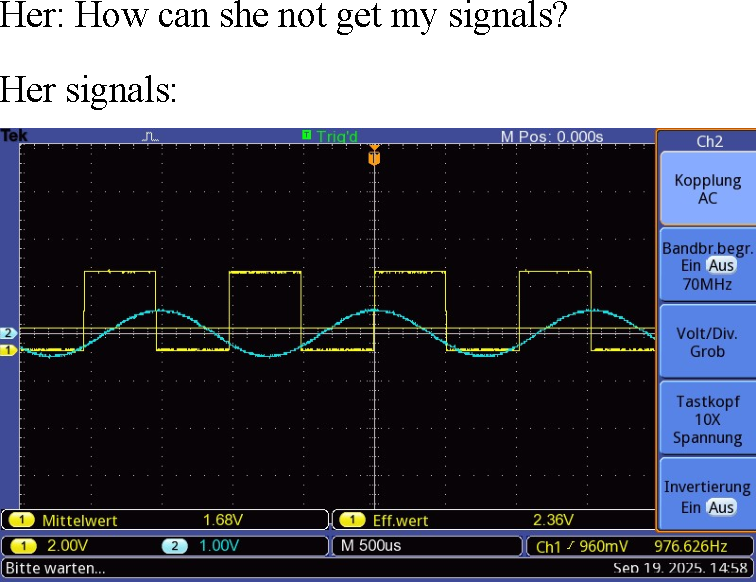
\includegraphics[width=0.4\textwidth]{img/25/memes/missedSignals.pdf}
    \caption{Noch ein meme}
\end{figure}

\section{Disskusion}
In diesem Teil wollen wir uns nun die Ergebnisse der Aufgaben anschauen und beurteilen, wie sinnvoll die Ergebnisse sind.
\subsection*{Aufgabe 1}
\subsubsection*{Signale 1 und 2}
\paragraph{Signal 1} Bei diesem Signal wurde einmal die DC-Offset-Spannung bestimmt:
\begin{equation}
    \boxed{
        U_{G} = (980 \pm 60) \, mV
    }
\end{equation}

und die Frequenz
\begin{equation}
    \underline{
        f_{cursor} = 0,2 ms^{-1} \, \hat= \, 5kHz
    }.
\end{equation}

Wir haben dann die berechneten Werte mit den gemessenen Werten verglichen, alle Ergebnisse sind wie zu erwarten in einer 1$\sigma$-Umgebung und gelten somit als statistisch signifikant.
Abweichung der Offset-Spannung
\begin{equation}
    \frac{\left| U_{G,auto} - U_{G,cursor} \right|}{\Delta U_{G,cursor}} = 0,83\sigma,
\end{equation}
der Frequenz
\begin{equation}
    \frac{\left| f_{auto} - f_{cursor} \right|}{\Delta f_{cursor}} = 0,33\sigma,
\end{equation}

und der Spitzen-Spitzen-Spannung
\begin{equation}
    \frac{\left| U_{SS,auto} - U_{SS,cursor} \right|}{\Delta U_{SS,cursor}} = 0,26\sigma.
\end{equation}
 
Das heißt für das Erste Signal konnte alle automatischen Messungen und alle Cursor-Messungen sich statistisch bestätigen.

\paragraph{Signal 2} Für dieses Signal wurden dieselben Werte bestimmt:
Die Frequenz
\begin{equation}
\boxed{
    f = (0,6410 \pm 0,0025) \, ms^{-1}
},
\end{equation}

die Offset-Spannung
\begin{equation}
\boxed{
    U_{G,cursor} = (63 \pm 6) \, mV
}
\end{equation}

und die Spitzen-Spitzen-Spannung
\begin{equation}
    \boxed{
        U_{SS,cursor} = (12 \pm 6) mV
    }.
\end{equation}

Hier werden die signifikanten Abweichungen jedoch interessant: 

Offset-Spannung:
\begin{equation}
    \frac{\left| U_{G,auto,2} - U_{G,cursor,2} \right|}{\sqrt{(\Delta U_{G,cursor,2})^2}} = 257,84\sigma
\end{equation}

Spitzen-Spitzen-Spannung:
\begin{equation}
    \frac{\left| U_{SS,auto,2} - U_{SS,cursor,2} \right|}{\sqrt{(\Delta U_{SS,cursor,2})^2}} = 15,33\sigma
\end{equation}

Für die Frequenz ließ sie sich gar nicht erst bstimmen. Wieso genau solche Abweichungen herauskamen kann ich nicht mit Garantie beantworten. Die offensichtlichste Idee ist, dass das automatische Messsystem mit dem stark schwankendem Signal nicht zureckt kam. So konnte beispielsweise die Periodendauer gar nicht erst automatisch bestimmt werden. Wieso genau jedoch das System des Osziloskopes hier ein Problem hat ist mir nicht erschließbar.

Es lässt sich damit jedoch zeigen, dass entweder die automatisch bestimmten Messwerte oder die mit dem Cursor bestimmten Messwerte einem systemischen Fehler unterliegen, der unbekannt ist.

Somit sollte das Osziloskop nicht für alle Signale als einwandfrei deklariert werden.

\subsubsection*{Signal 5}
Die Rechnung war alles andere als kompliziert, wir kamen auf ein Ergebnis von
\begin{equation}
\boxed{
    t_H = (2,40 \pm 0,15)\, ms
}.
\end{equation}

Diese Werte lassen sich mit einem Blick auf das Display recht schnell bestätigen, da dies gerade ca eine Div-Größe ist.
Einen Vergleichswert gibt es nicht.

\subsubsection*{Signal 9}
Dies wurde wieder interessanter, denn hier gab es einiges zurechnen. Zunächst wurden die Schwinungsperiode $T_1$ und die Schwebunsgperiode $T_2$ bestimmt:
\begin{equation}
\boxed{
    T_1 = (0,660 \pm 0,006) \, ms
},
\end{equation}

\begin{equation}
\boxed{
    T_{2} = (9,95 \pm 0,16) \, ms
}.
\end{equation}


Aus diesen konnten die Frequenzen $f_1$ und $f_2$ bestimmt werden:
\begin{equation}
\boxed{
    f_1 = (1,515 \pm 0,014) \, ms^{-1}
},
\end{equation}
\begin{equation}
\boxed{
    f_2 = (0,101 \pm 0,016) \, ms^{-1}
}.
\end{equation}

Dabei ist $T_2$ um einiges Größer als $T_1$. Dies ist plausibel, da $T_2$ die Periode der Umhüllenden ist, sie umhüllt also die Perioden der Schwinungen. Wir müssten also sehen, dass die Summe der Schwinungen, die in der Umhüllenden liegen gerade der Periodendauer der Schwebung sind. Zählt man die Perioden graphisch ab, so kommt man auf 15 Schwinungsperioden pro Schwebungsperiode. Rechhnerisch prüfen:
\begin{equation}
    9,95 \div 0,66 = 15,076.
\end{equation}
Wir sehen also, die Ergebnisse decken sich gegenseitig sehr gut.

Darüber hinaus sollten noch die spezifischen Eigenschwinungen der beiden Sinuskurven bestimmt werden, die das Schwebunsgsignal bilden. Dies wurde im FFT-Modus getan. Das Ergebnis war dann
\begin{equation}
    \boxed{
        f_{i} = (1390,00 \pm 1,25) Hz
    },
\end{equation}
\begin{equation}
    \boxed{
        f_{ii} = (1590,00 \pm 1,25) Hz
    }
\end{equation}

Wir wollen die Plausibilität wieder Prüfen. Die Schwebunsgsfrequenz ist gerade die Differenz der beiden spezifischen Eigenfrequenzen:
\begin{equation}
    \left| f_i - f_{ii} \right| = 200Hz \hat = 0,2ms^{-1}.
\end{equation}

Der Fehler der Addition ist:
\begin{equation}
    \sqrt{(\Delta f_i )^2 + (\Delta f_{ii})^2} = 0,00176ms^{-1}.
\end{equation}

Erwartet hätten wir einen Wert von $f_2 = 0,1ms$. 

Die Abweichung beträgt:
\begin{equation}
    \frac{\left| 0,2ms^{-1} - 0,101ms^{-1} \right|}{\sqrt{(0,00176ms^{-1})^2 + (0,016ms^{-1})^2}} = 6,15\sigma.
\end{equation}

Selbiges können wir für die Schwinnugnsfrequenz machen, diese ist gerade der Mittelwert der beiden Eigenfrequenzen:
\begin{equation}
\frac{f_i + f_{ii}}{2} = 1490 Hz \hat = 1,49 ms^{-1}.
\end{equation}

Der Fehler ist dabei wieder $\Delta f_{i+ii} = 0,00176ms^{-1}$.

Erwartet hätten wir den Wert von 1,515. Wir schauen uns die Abweichung zu $f_1$ an:
\begin{equation}
\frac{\left| 1,49 ms^{-1} -  1,515 ms^{-1} \right|}{\sqrt{(0,00176ms^{-1})^2 + (0,014ms^{-1})^2}} = 1,77\sigma.
\end{equation}

Es zeigt sich also, die Messergebnisse im FFT-Modus sind nicht konsistent mit dem YT-Modus.

\subsection*{Aufgabe 3}
In dieser Aufgabe wurden die Pulse zweier Pulse beobachtet. Die berechneten Spannungen sind für den Ersten Puls:
\begin{equation}
\boxed{
    U_{avg,r} = (1,775 \pm 0,040) \, V
},
\end{equation}
und 
\begin{equation}
    \boxed{
        U_{eff} = (2,49 \pm 0,06) V
    }.
\end{equation}

Für das zweite Signal:
\begin{equation}
    \boxed{
        U_{avg,r,2} = (0,878 \pm 0,019) \, V
    }
\end{equation}
und 
\begin{equation}
    \boxed{
        U_{eff,r,2} = (1,73 \pm 0,04) \, V
    }.
\end{equation}


Auffällig ist, dass die Durchschnittsspannung des ersten Pulses ca. doppelt so groß ist, seine Effektivspannung jedoch nur 1,44 mal so groß. Dies liegt offensichtlich an der Wurzelbeziehung. Dies hat jedoch auch zur Folge, dass die LED nicht doppelt so stark in ihrer itensität abgenommen hat, sie hatte noch kanpp 70\% der Leuchtkaft.

Wir haben außerdem die Messwerte mit den berechneten Werten bestimmt, für das erste Signal decken sich alle Ergebnisse statistisch:
\begin{equation}
    \frac{\left| U_{avg} - U_{avg,r} \right|}{\sqrt{(\Delta U)^2 + (\Delta U_{avg,r})^2}} = 0,52\sigma,
\end{equation}

\begin{equation}
    \frac{\left| U_{eff} - U_{eff,r} \right|}{\sqrt{(\Delta U)^2 + (\Delta U_{eff,r})^2}} = 0,41\sigma.
\end{equation}

Bei dem zweiten Signal jedoch nicht:
\begin{equation}
    \frac{\left| U_{avg,2} - U_{avg,r,2}\right|}{\sqrt{(\Delta U)^2 + (\Delta  U_{avg,r,2})}} = 2,17\sigma,
\end{equation} 

\begin{equation}
    \frac{\left| U_{eff,2} - U_{eff,r,2}\right|}{\sqrt{(\Delta U)^2 + (\Delta  U_{eff,r,2})}} = 1,96\sigma.
\end{equation} 

Woran das liegt kann ich mir nicht erklären, außer es liegt an Messungenauigkeiten. Eigentlich wäre eine geringere Abweichung zu vermuten, da die Fehler größer im Verhältnis zu den Messwerten sind, was sich positiv auf die Abweichung auswirkt. 

\subsection*{Aufgabe 4}
In dieser Aufgabe sollte die Kabellänge bestimmt werden und der Wellenwiderstand geprüft.

Die Länge des Kabels kam auf einen Wert von: 
\begin{equation}
\boxed{
    L = (18,6 \pm 0,6) \, m
}
\end{equation}

was stark von den erwarten 25 Metern abweicht. Vermutlich ist das Kabel aber tatsächlcih eher ca. 19 Meter lang.

Die statistische Abweichung liegt dabei bei
\begin{equation}
    \frac{\left| 25m-18,6m \right|}{0,6m} = 10,67\sigma.
\end{equation}

Bei dem innenwiderstand kommen wir auf ähnlich stark abweichende Werte. Mit dem gemessenen Widerstand von 38,8$\Omega$, betrug die Abweichugn $11,7\sigma$.

Entweder wir haben den Widerstand falsch bestimmt (zum Beispiel könnte er bei 48,3$\Omega$ liegen), oder der Fehler des Geräter ist eigentlich größer. So wäre eine Abweichung von:
\begin{equation}
    \frac{\left| 50 \Omega - 48,3 \Omega  \right|}{2 \Omega} = 0,85\sigma
\end{equation}
möglich.

Die alternative ist, dass unsere Messwere korrekt sind, und das Kabel tatsächlich eigentlich bei eher $40\Omega$ liegt. Ohne weitere Test sollten beide Aussagen als gleich plausibel angenommen werden.

\section{Kritik}

Bei der Kritik kann man sich kurz halten, jegliche Fehlerquellen lassen sich auf das Osziloskop zurückführen, bessere Technik würde die Werte genauer bestimmen. Natürlich wäre auch das anlegen größerer Messreihen sinnvoll gewesen, da so die Wahrscheinlichkeit für ausreißerwerte sinkt, beziehungsweise diese nicht so schwerwigend sind.

\begin{figure}[h!]
    \centering
    
\includegraphics[width=0.3\textwidth]{img/25/memes/ergebnisse.pdf}
    \caption{Wieder ein Meme}
\end{figure}